\documentclass[aspectratio=169]{beamer}

\usepackage{graphicx}

\usetheme{Madrid}
\usecolortheme{default}

\title{Emergency Services Communication Platform}
\subtitle{Project Progress Recap}
\author{CE1 Group 3}
\date{}

\begin{document}

\begin{frame}
    \titlepage
\end{frame}

\begin{frame}{Recap}
    \begin{block}{Project goal}
        Provide a shared communication interface for emergency services.
    \end{block}

    \vfill

    The platform acts as a centralized communication layer between emergency-service users and systems.
\end{frame}

\begin{frame}{Architecture}
    \begin{columns}[T]
        \begin{column}{0.48\textwidth}
            \textbf{Before}
            \begin{itemize}
                \item Single-node Kubernetes cluster
                \item Hosted with Minikube
            \end{itemize}
        \end{column}
        \begin{column}{0.48\textwidth}
            \textbf{Now}
            \begin{itemize}
                \item Multi-node Kubernetes cluster (k3s)
                \item Three worker nodes
                \item Managed with \texttt{kubectl}
                \item Portainer.io used for visualization
            \end{itemize}
        \end{column}
    \end{columns}
\end{frame}

\begin{frame}{Current Cluster Layout}
    \begin{block}{Physical machine 1}
        Control plane + one worker node running in a virtual machine.
    \end{block}

    \begin{block}{Physical machine 2}
        Two worker nodes running in virtual machines.
    \end{block}

\end{frame}

\begin{frame}{Cluster Overview}

    \begin{center}
            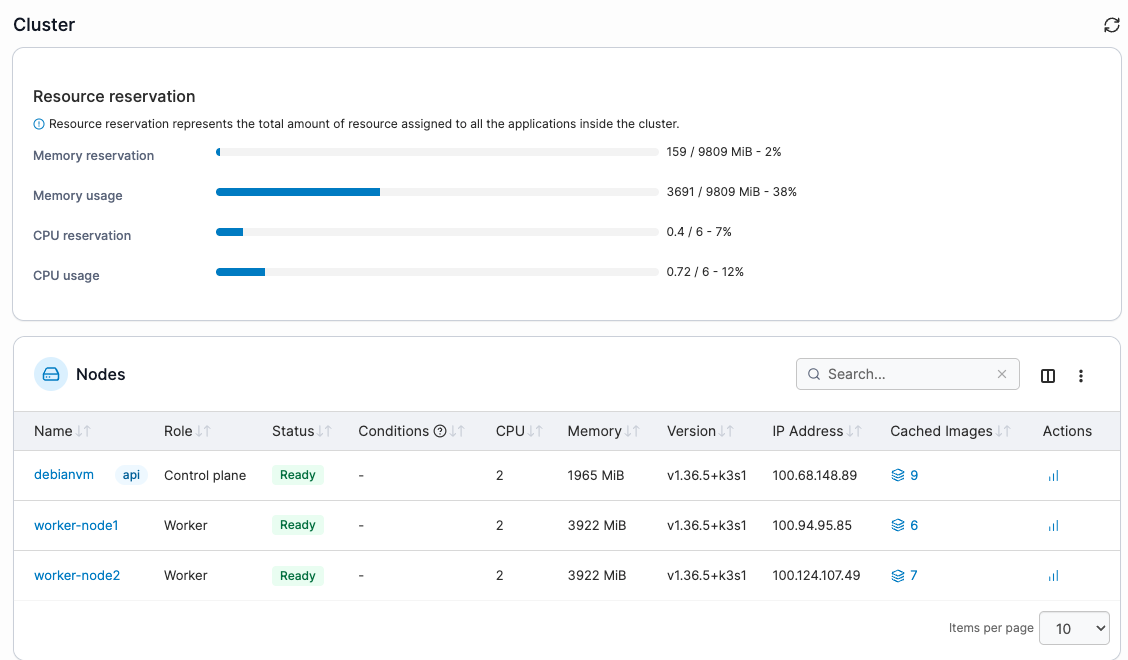
\includegraphics[width=0.75\linewidth]{./img/Screenshot_2026-10-26_at_11.52.32_PM.png}
    \end{center}
\end{frame}

\begin{frame}{Data layer}
    \begin{columns}[T]
        \begin{column}{0.38\textwidth}
            \textbf{Data}
            \begin{itemize}
                \item Database schemas established.
                \item Basic database queries established.
            \end{itemize}
        \end{column}
        \begin{column}{0.58\textwidth}
            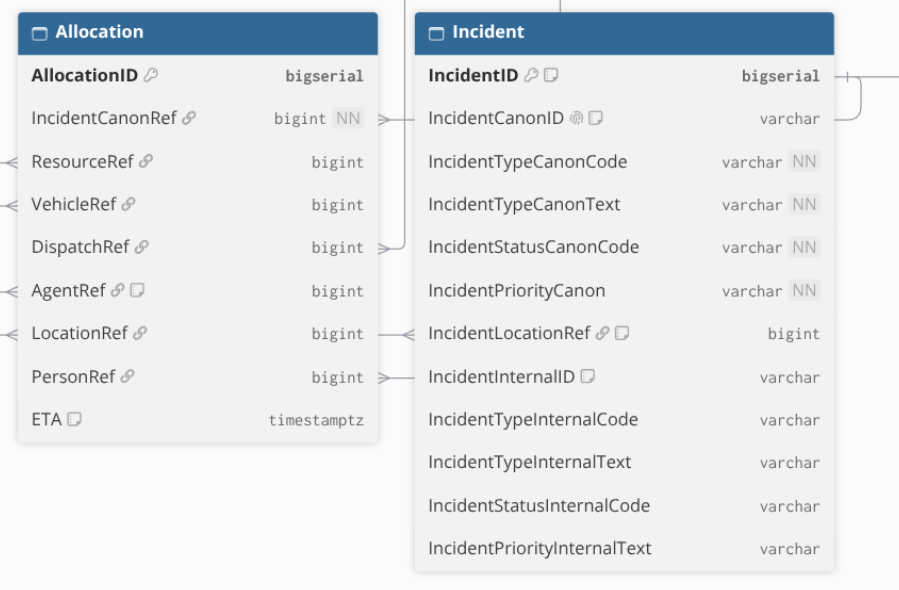
\includegraphics[width=\linewidth]{./img/2026-10-26 17-01-28_1.png}
        \end{column}
    \end{columns}
\end{frame}

\begin{frame}{Domain}
    \begin{itemize}
        \item Incident model established.
        \item Business rules for incidents established.
        \item Valid incident state transitions defined.
    \end{itemize}

    \vfill

    \begin{block}{Result}
        Incident behavior is constrained by explicit domain rules rather than arbitrary status updates.
    \end{block}
\end{frame}


\begin{frame}{Application}
    \begin{columns}[T]
        \begin{column}{0.46\textwidth}
            \begin{itemize}
                \item API adapted to the incident domain.
                \item Basic CRUD operations are implemented.
                \item Seperation of concerns
            \end{itemize}
        \end{column}
        \begin{column}{0.50\textwidth}
            \begin{itemize}
                \item Transport $\leftrightarrow$ Application
                \item Application $\leftrightarrow$
                  \begin{itemize}
                    \item Domain 
                    \item Repository (ORM) 
                  \end{itemize}
            \end{itemize}
        \end{column}
    \end{columns}
\end{frame}

\begin{frame}{Next Focus}
    \begin{enumerate}
        \item Backend - API - WebSocket
        \item Frontend - UI
        \item Report
    \end{enumerate}
\end{frame}

\end{document}
